\chapter{Related Works}

Your related works, and your purpose and contribution which must be different as below.

\section{Cokro Edi Prawiro/ 1164069}

\subsection{Teori}
\begin{enumerate}
\item Jelaskan Apa Itu binari calssification drlengkapi ilustrasi gambar sendiri.\par
Binary Classification atau biominal adalah tugas mengklasifikasikan unsur usur dari himpunan yang diberikan kedalam kedua kelompok berdasarkan aturan klasifikasi yang telah ditetapkan. binari clasification juga dapat diartikan sebagai pembagi yang hanya memberikan dua pilihan contohnya benar dan salah atau klasifikasi tongkat panjang atau pendek. penjelasan lebih singkatnya binari classification merupakan kegiatam mengkelasifikasikan yang hanya memberikan dua class. contoh pada gambar \ref{c10} clasifikasi antara betuk kotak dan segitiga.

\item Jelaskan Apaitu supervised learning , unsupervised learning dan clusterring dengan ilustrasi gambar sendiri.\par
supervised learning adalah cara untuk mengklasifikasikan suatu objek atau data yang telah di tentukan kelas kelasnya contoh pada sayuran tumbuhan wortel termasuk yang mengandung vitamin A berarti tumbuhan wortel telah di kategorikan kedalam sayuran yang mengandung vitamin A. sedangkan kangkung mengandung zat besi yang berarti tumbuhan kangkung telah di kategorikan kedalam sayuran yang mengandung zat besi untuk lebih jelasnya dapat dilihat pada gambar \ref{c11}.\par
unsupervised learning merupakan cara untuk mengklasifikasi tanpa adanya kelas untuk menentukan jenisnya contoh sayuran berarti semua objek yang memiliki ciri ciri sayuran di kategorikan kedalam sayuran untuk lebih jelasnya dapat dilihat pada gambar \ref{c12}.\par
clustering merupakan peroses mengklasifikasikan yang berdasarkan suatu parameter dalam penentuannya contoh pada berat sayuran sayuran A memiliki berat 100 gr dan sayuran B memiliki berat 120 gr yang berarti berat sayuran dibagi dua parameter yaitu lebih kecil samadengan 100 gram dan lebih besar dari gram contoh pada gambar \ref{c13}.\par

\item Jelaskan apa itu evaluasi dan akurasi dan disertai ilustrasi contoh dengan gambar sendiri.\par
evaluasi adalah pengumpulan pengumpulan dan pengamatan dari berbagai macam bukti untuk mengukur dampak efektifitas dari suatu objek, program, atau proses berkaitan  dengan spesifikasi atau persyaratan yang telah di tetapkan sebelumnya. sedangkan akurasi itu sndiri merupakan bagian dari evaluasi yang merupakan ketepatan data terhadap suatu objek berdasarkan keriteria tertentu. kita dapat mengevaluasi seberapa baik model bekerja dengan mengukur akurasinya. ketepatan akan di definisikan sebagai presentase kasus yang di klasifikasikan dengan benar. hal ini berkaitan dengan confusion matrix pada materi selanjutnya. contoh evaluasi untuk membedakan burung dengan ayam terdapat parameter yaitu ukuran badan dan fungsi sayap pada hewan tersebut. lebih jelanya pada gambar \ref{c14} berikut:

\item Jelaskan bagaimana cara membuat Confusion Matrix, Buat confusion matrix sendiri.\par
Dalam pembuatan confusion matrix tentukan parameter atau objek yang akan di evaluasi contoh bunga melati , bunga mawar, dan bunga kenangan buat tabel dengan baris dan kolom berjumlah tiga kemudian tentukan nilai miring pada setiap kolom tersebut disini saya memberi nilai 30 dengan ketentuan setiap baris harus berisi nilai 30 nilai tersebut jika terbagi ke kolom lain maka jumlahnya harus bernilai 30 jika tidak berarti data tersebut tidak akurat. untuk lebih jelanya dapat dilihat pada gambar \ref{c15} berikut :

\item Jelaskan bagaimana K-fold cross validation bekerja dengan gambar ilustrasi contoh buatan sendiri.
K-fold Cross Validation merupakan cara untuk melatih suatu mesin dimana di dalammya terdapat data set yang dibagi menjadi dua yaitu untuk data testing dan data training contoh 1000 data merupakan data set dan 200 data digunakan untuk data testing kemudian 800 datanya digunakan untuk data training dimana data training tersebut digunakan untuk menentukan nilai bobot yang dimasukan kedalam rumus regresi linier. sedangkan nilai testing akan dijadikan nili inputan untuk rumus regresi linier. contohnya dapat dilihat pada gambar \ref{c16}  berikut :

\item Jelaskan Apa itu decision tree dengan gambar ilustrasi contoh buatan sendiri.\par
Decision tree (pohon keputusan) merupakan implementasi dari binari clasification dimana pada pohon keputusan akan terdapat root atau akar dan cabang cabangnya yang nilainya seperti if contoh pada root berisi nilai jenis kelamin, apakah perempuan pada cabang satu bernilai iya dan pada cabang dua bernilai tidak jika nilainya iya berarti jenis kelamminya perempuan dan jika tidak maka bernilai laki-laki.
agar lebih jelas dapat dilihat pada gambar \ref{c17}  decision tree berikut:

\item jelaskan apa itu information gain dan entropi dengan gambar ilustrasi buatan sendiri.\par
informasion gain merupakan informasi atau keriteria dalam pembagian sebuah objek contoh information gain pada laki-laki yaitu berrambut pendek, memiliki jakun, berjenggot, berkumis, dan mempunyai bahu yang lebar. pada kriteria tersebut seringkali terdapat bias misalkan ada perempuan yang berrambut pendek atau berkumis namun dari parameter tersebut dapat dilihat bahwa 60 persen parameter tersebut tepat pada sasaranya selama parameter itu bernilai tinggi untuk tepat maka dapat digunakan itulah information gain untuk lebih jelasnya dapat dilihat pada gambar \ref{c18}  berikut :\par
sedangkan entropi merupakan ukuran keacakan dari informasi semakin tinggi entropi maka semakin sulit dalam menentukan keputusan contoh dalam menentukan jenis kelamin semakin detail informasi maka akan semakin susah dalam menentukan keputusan.
\end{enumerate}


\subsection{Topic 2}
if you have two topics you can include here to


\section{Same Method}
write and cite latest journal with same method

\subsection{Method 1}
cite and paraphrase method 1

\subsection{Method 2}
cite and paraphrase method 2 if you have more method please add new subsection.

\section{Ahmad Syafrizal Huda/1164062}
\subsection{Teori}
\begin{enumerate}
\item Binary Classification yaitu katakanlah kita memiliki tugas untuk mengklasifikasikan objek menjadi dua kelompok berdasarkan beberapa fitur. Sebagai contoh, katakanlah kita diberi beberapa pena dan pensil dari berbagai jenis dan merek, kita dapat dengan mudah memisahkannya menjadi dua kelas, yaitu pena dan pensil.
\subitem Contoh ilustrasi gambar bisa dilihat pada gambar \ref{1}.

\item Supervised learning merupakan sebuah pendekatan dimana sudah terdapat data yang dilatih, dan terdapat variable yang ditargetkan sehingga tujuan dari pendekatan ini adalah mengkelompokan suatu data ke data yang sudah ada. Sedangkan unsupervised learning tidak memiliki data latih, sehingga dari data yang ada, kita mengelompokan data tersebut menjadi 2 bagian atau 3 bagian dan seterusnya. Dan clustering adalah proses pengelompokan entitas yang sama bersama-sama. Tujuan dari teknik pembelajaran mesin tanpa pengawasan ini adalah untuk menemukan kesamaan pada titik data dan mengelompokkan titik data yang serupa secara bersamaan\cite{zhu2009introduction}.
\subitem Contoh ilustrasi gambar bisa dilihat pada gambar \ref{2}.
\subitem Contoh ilustrasi gambar bisa dilihat  pada gambar \ref{3}.
\item Evaluasi dan akurasi adalah bagaimana cara kita bisa mengevaluasi sebarapa baik model mengerjakan pekerjaannya dengan cara mengukur akurasinya. Akurasi nantinya didefinisikan sebagai presentase kasus yang telah diklasifikasikan dengan benar. Kita dapat melakukan analisis kesalahan yang telah di buat oleh model.
\subitem Contoh ilustrasi gambar bisa dilihat pada gambar \ref{5}.
\item Cara membuat dan membaca confusion matrix yaitu, menentukan pokok permasalahan serta atributnya, membuat Decision Tree, membuat Data Testing, mencari nilai variabelnya misal a,b,c, dan d, mencari nilai recall, precision, accuracy, dan erorr rate.
\subitem Contoh Confusion Matrix.
\begin{verbatim}
		Recall =3/(1+3) = 0,75
		Precision = 3/(1+3) = 0,75
		Accuracy =(5+3)/(5+1+1+3) = 0,8
		Error Rate =(1+1)/(5+1+1+3) = 0,2 
\end{verbatim}
\item Berikut ini tata cara kerja K-fold Cross Validation>
	\begin{itemize}
		\item Total instance akan dibagi menjadi N bagian.
		\item Fold yang pertama adalah bagian pertama menjadi testing data dan sisanya menjadi training data.
		\item Hitung akurasi berdasarkan porsi data tersebut dengan menggunakan persamaan.
		\item Fold yang ke dua adalah bagian ke dua menjadi testing data dan sisanya training data. 
		\item Hitung akurasi berdasarkan porsi data tersebut.
		\item Lakukan step secara berulang hingga habis mencapai fold ke-K.
		\item Terakhir hitung rata-rata akurasi K buah.
	\end{itemize}
\subitem Contoh ilustrasi gambar bisa dilihat pada gambar \ref{6}.
\item Decision Tree adalah sebuah metode pembelajaran yang digunakan untuk melakukan klarifikasi dan regresi. Decision Tree digunakan untuk membuat sebuah model yang dapat memprediksi sebuah nilai variabel target dengan cara mempelajari aturan keputusan dari fitur data. Contoh Decision Tree adalah untuk melakukan predikisi apakah Kuda termasuk hewan mamalia atau bukan.
\subitem Contoh ilustrasi gambar bisa dilihat pada gambar \ref{7}.
\item Gain adalah pengurangan yang diharapkan dalam enthropy. Dalam mechine learning, gain dapat digunakan untuk menentukan sebuah urutan atribut atau memperkecil atribut yang telah dipilih. Urutan ini akan membentuk decision tree, atribut gain dipilih yang paling besar. Dan Entropi adalah ukuran ketidakpastian sebuah variabel acak sehingga dapat di artikan entropi adalah ukuran ketidakpastian dari sebuah atribut.
\subitem Contoh ilustrasi gambar bisa dilihat pada gambar \ref{8}.
\end{enumerate}

\begin{figure}[ht]
		\centerline{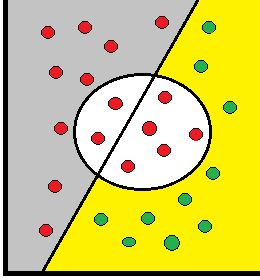
\includegraphics[width=1\textwidth]{figures/huda/binary.JPG}}
		\caption{Binary Classification.}
		\label{1}
\end{figure}
\begin{figure}[ht]
		\centerline{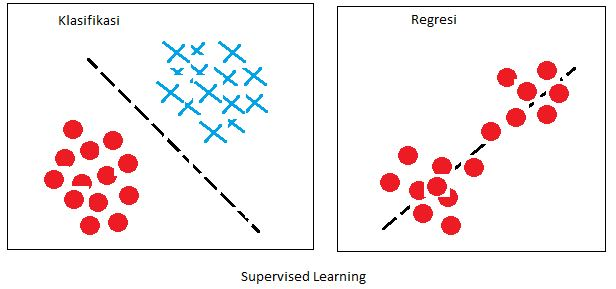
\includegraphics[width=1\textwidth]{figures/huda/supervised.JPG}}
		\caption{Supervised Learning.}
		\label{2}
\end{figure}
\begin{figure}[ht]
		\centerline{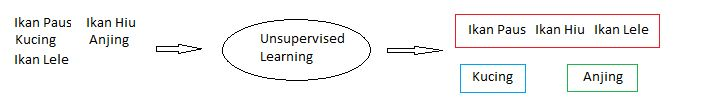
\includegraphics[width=1\textwidth]{figures/huda/unsupervised.JPG}}
		\caption{Unsupervised Learning.}
		\label{3}
\end{figure}
\subitem Contoh ilustrasi gambar bisa dilihat pada gambar \ref{4}.
\begin{figure}[ht]
		\centerline{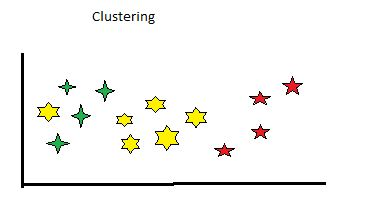
\includegraphics[width=1\textwidth]{figures/huda/clustering.JPG}}
		\caption{Clustering.}
		\label{4}
\end{figure}
\begin{figure}[ht]
		\centerline{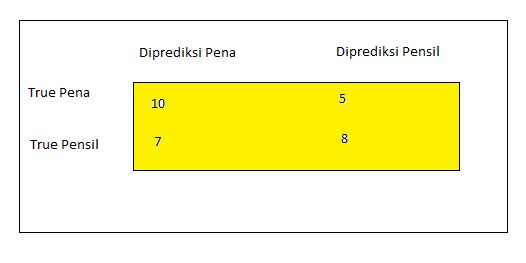
\includegraphics[width=1\textwidth]{figures/huda/evaluasidanakurasi.JPG}}
		\caption{Evaluasi dan Akurasi.}
		\label{5}
\end{figure}
\begin{figure}[ht]
		\centerline{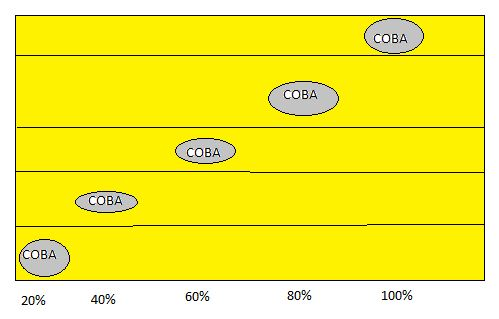
\includegraphics[width=1\textwidth]{figures/huda/K-fold.JPG}}
		\caption{K-fold Cross Validation.}
		\label{6}
\end{figure}
\begin{figure}[ht]
		\centerline{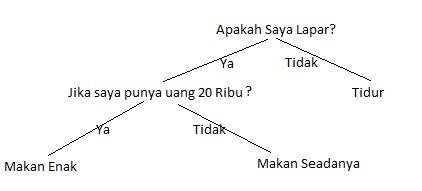
\includegraphics[width=1\textwidth]{figures/huda/DecisionTree.JPG}}
		\caption{Decision Tree.}
		\label{7}
\end{figure}
\begin{figure}[ht]
		\centerline{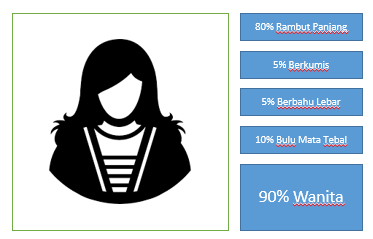
\includegraphics[width=1\textwidth]{figures/huda/Gain.PNG}}
		\caption{Gain.}
		\label{8}
\end{figure}

\begin{figure}[ht]
      \centerline{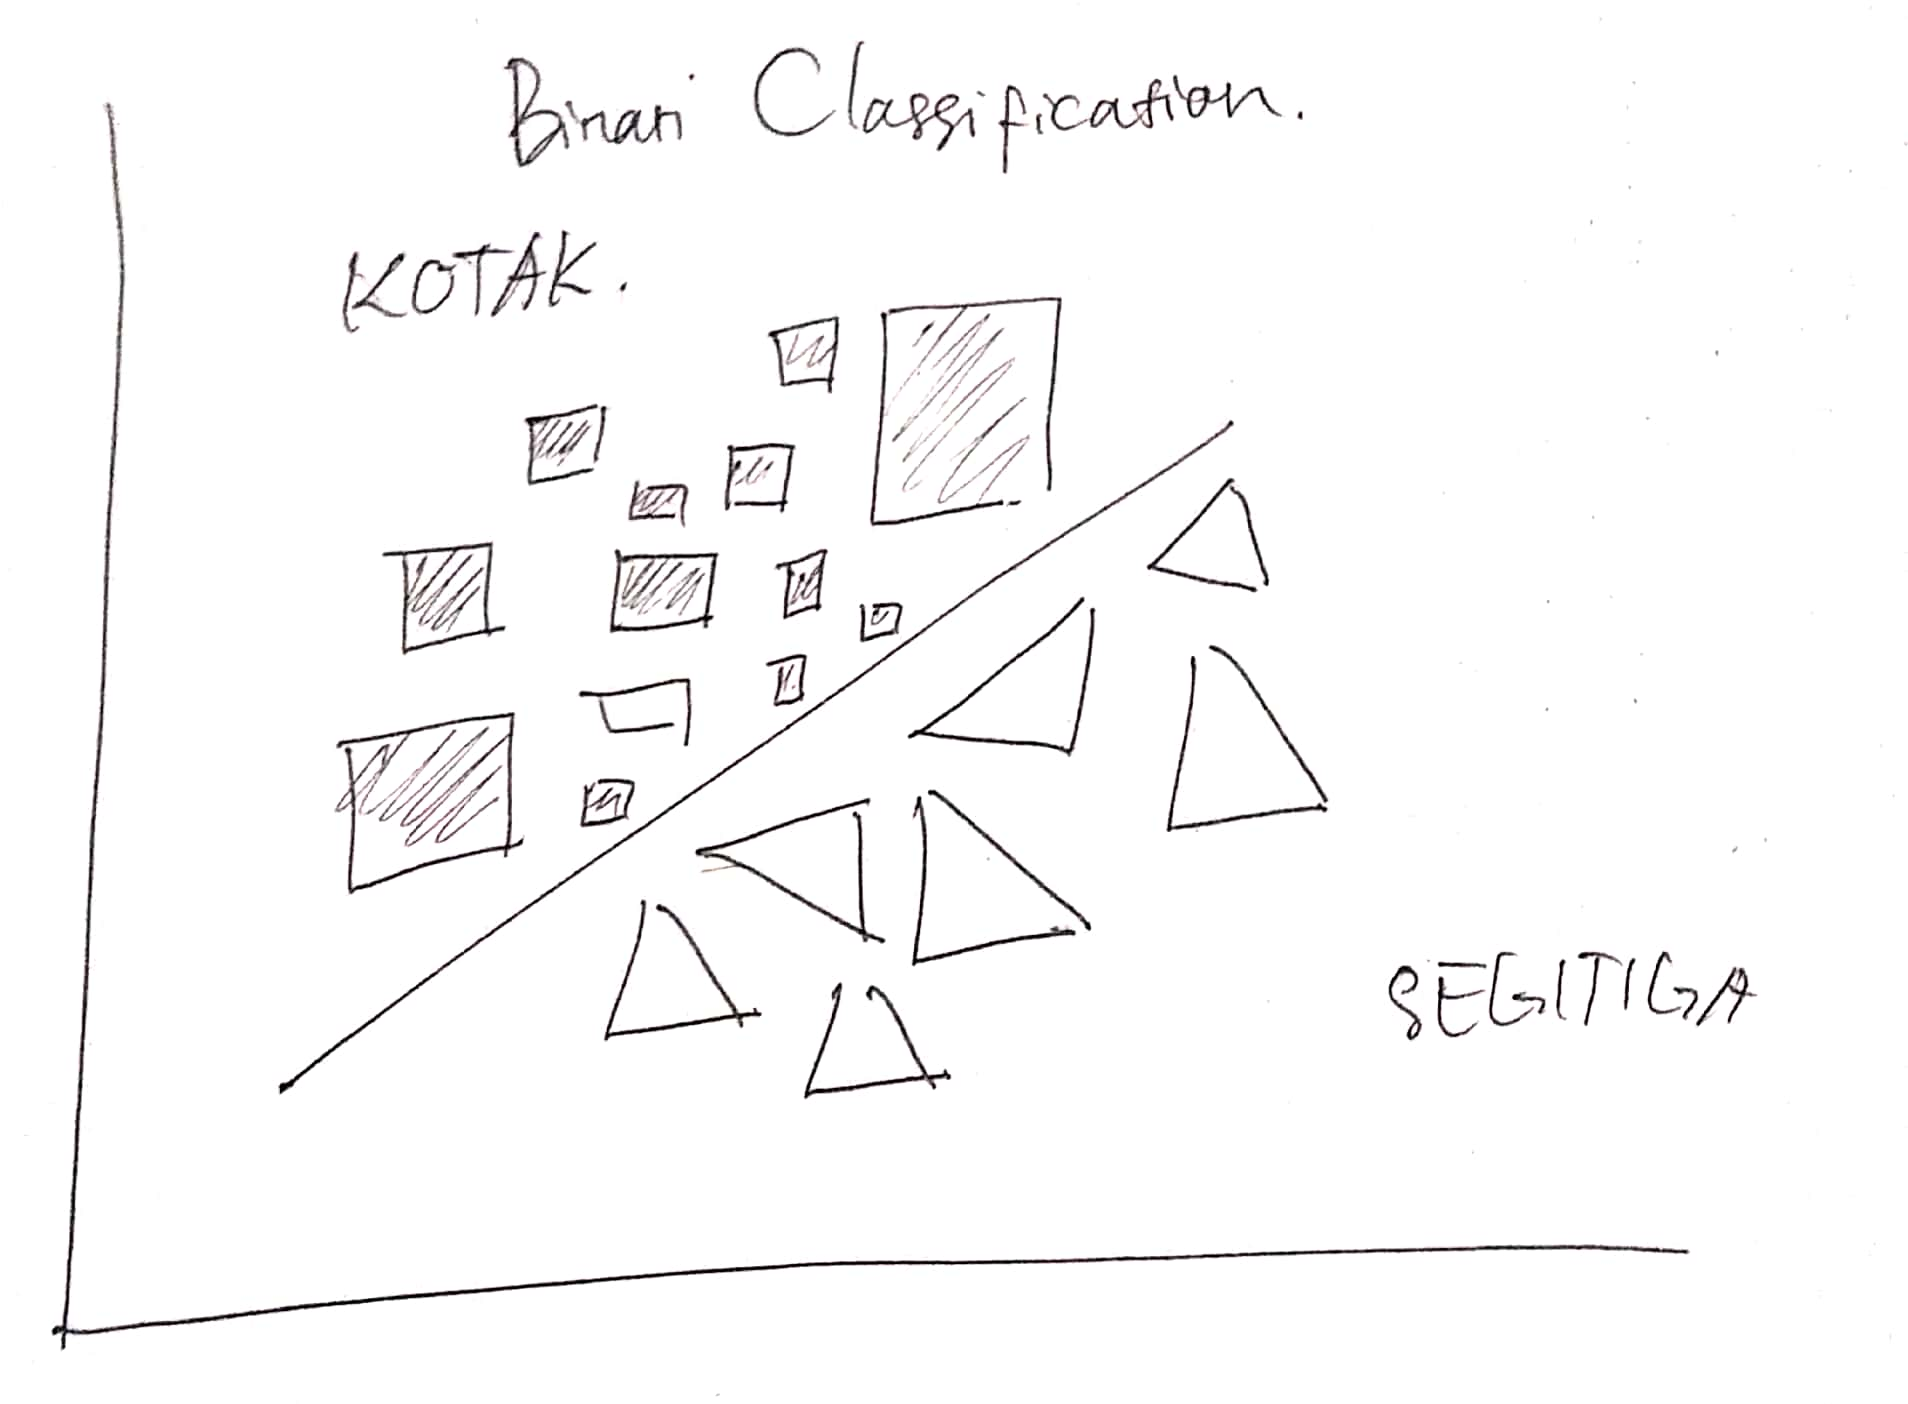
\includegraphics[width=1\textwidth]
      {figures/c10}}
      \caption{Contoh Binary Classification}
      \label{c10}
      \end{figure}

\begin{figure}[ht]
      \centerline{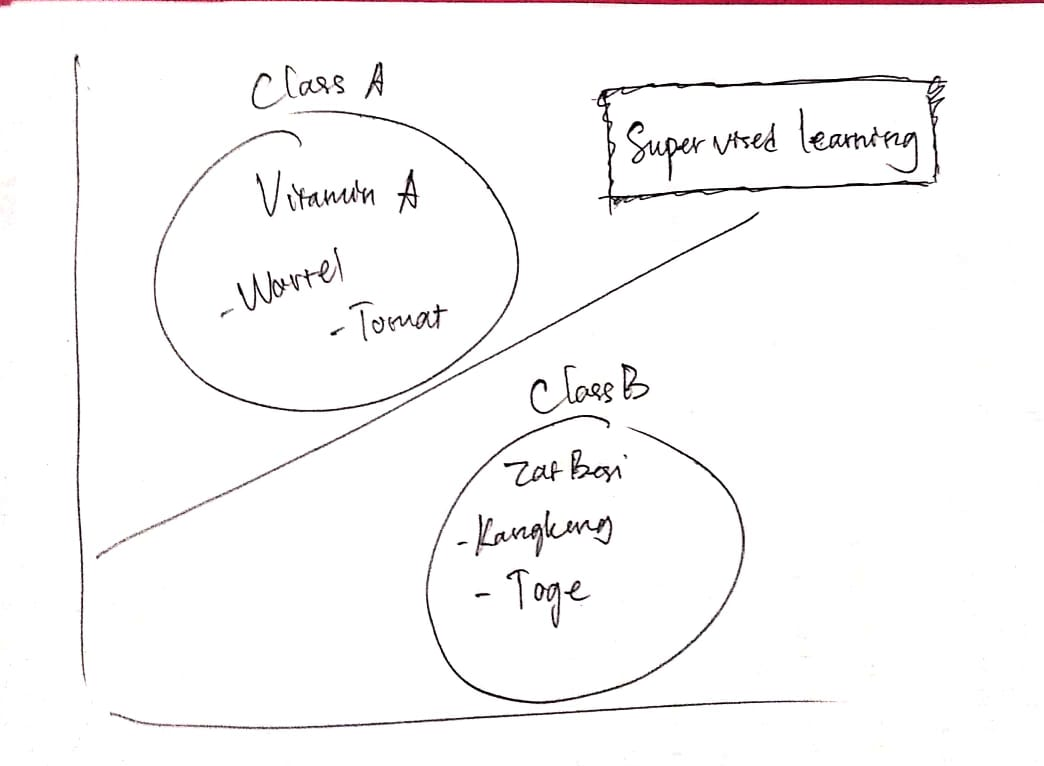
\includegraphics[width=1\textwidth]
      {figures/c11}}
      \caption{Contoh Binary Classification}
      \label{c11}
      \end{figure}

\begin{figure}[ht]
      \centerline{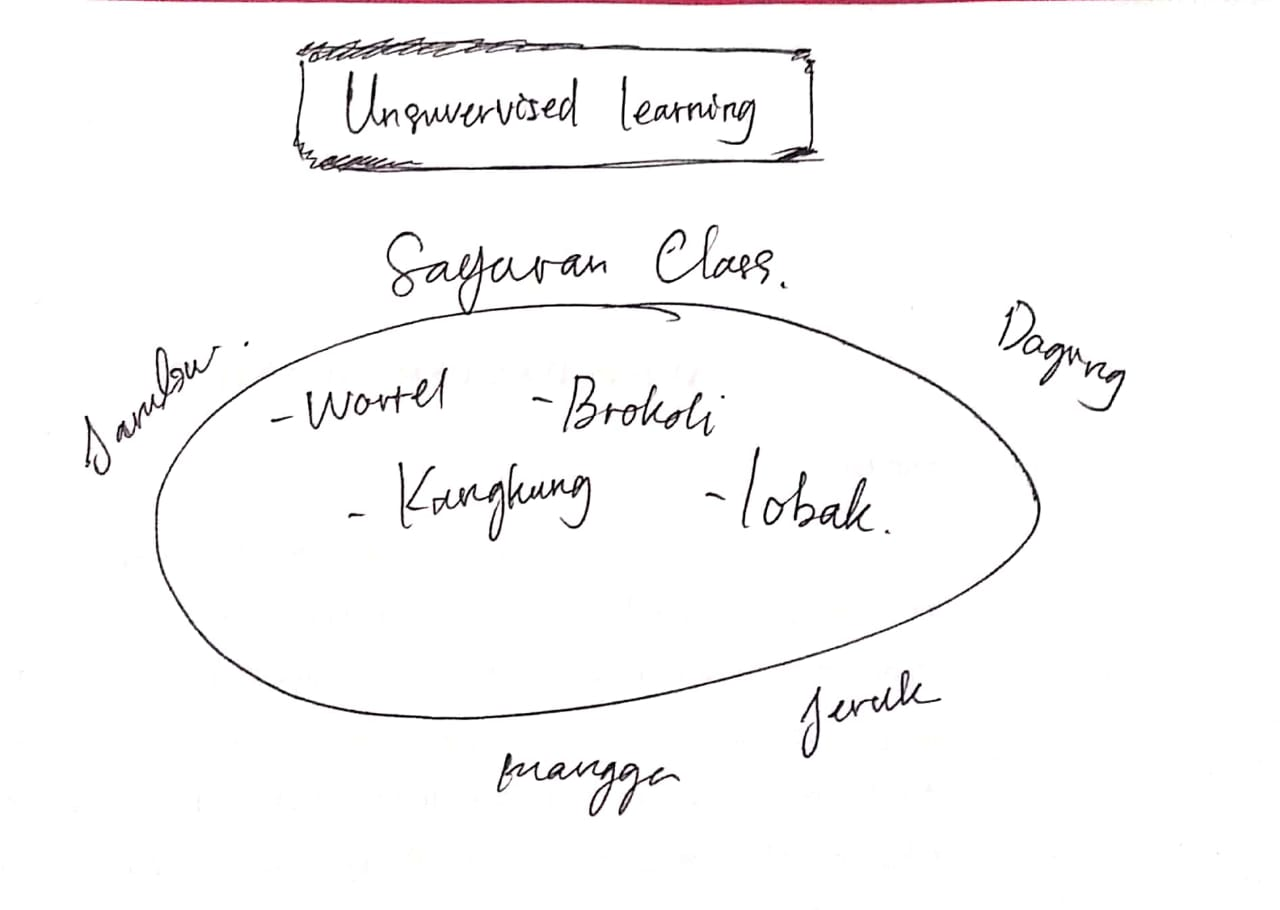
\includegraphics[width=1\textwidth]
      {figures/c12}}
      \caption{Contoh Binary Classification}
      \label{c12}
      \end{figure}

\begin{figure}[ht]
      \centerline{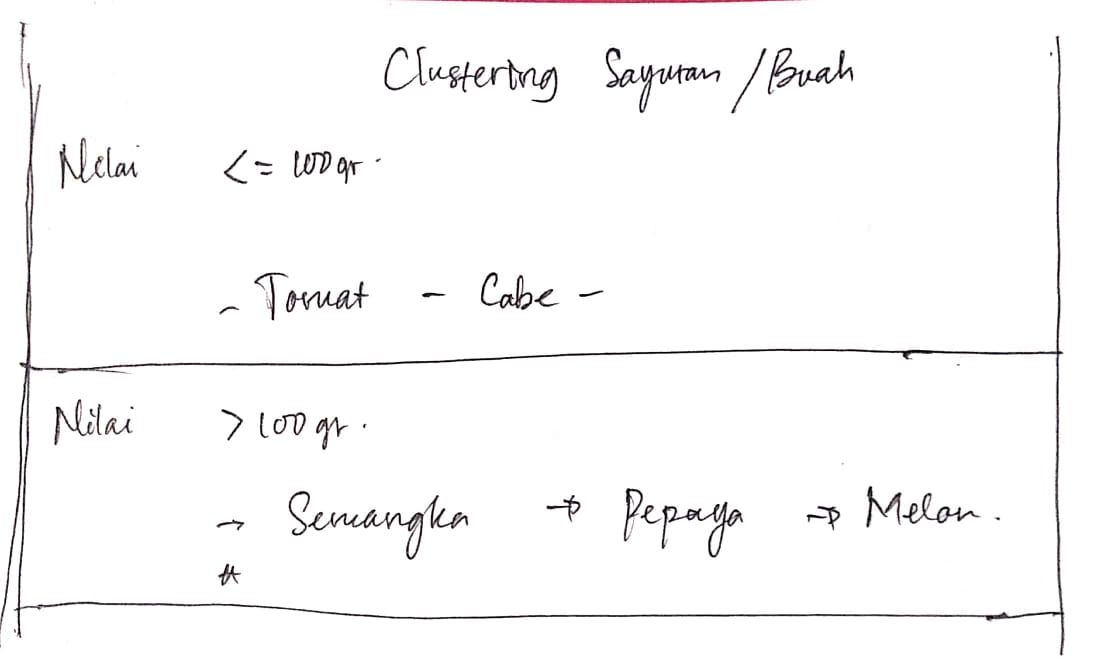
\includegraphics[width=1\textwidth]
      {figures/c13}}
      \caption{Contoh Binary Classification}
      \label{c13}
      \end{figure}

\begin{figure}[ht]
      \centerline{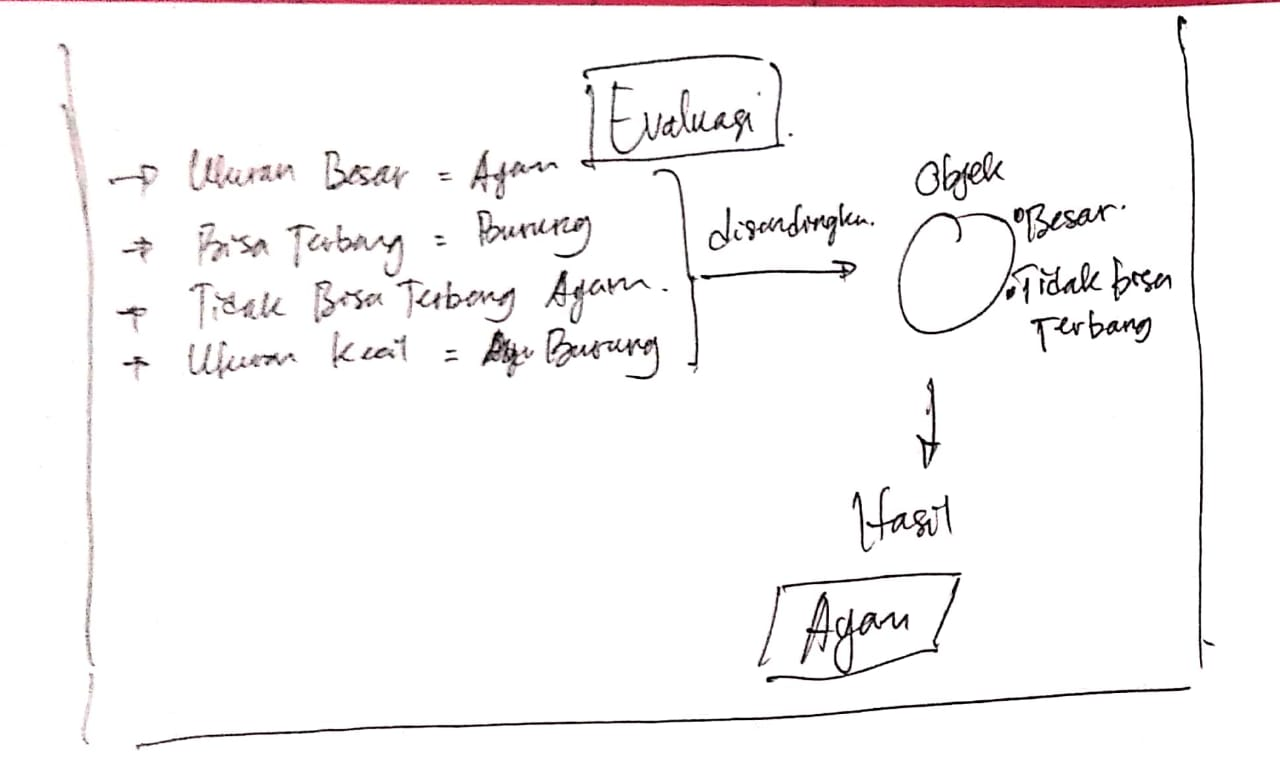
\includegraphics[width=1\textwidth]
      {figures/c14}}
      \caption{Contoh Binary Classification}
      \label{c14}
      \end{figure}

\begin{figure}[ht]
      \centerline{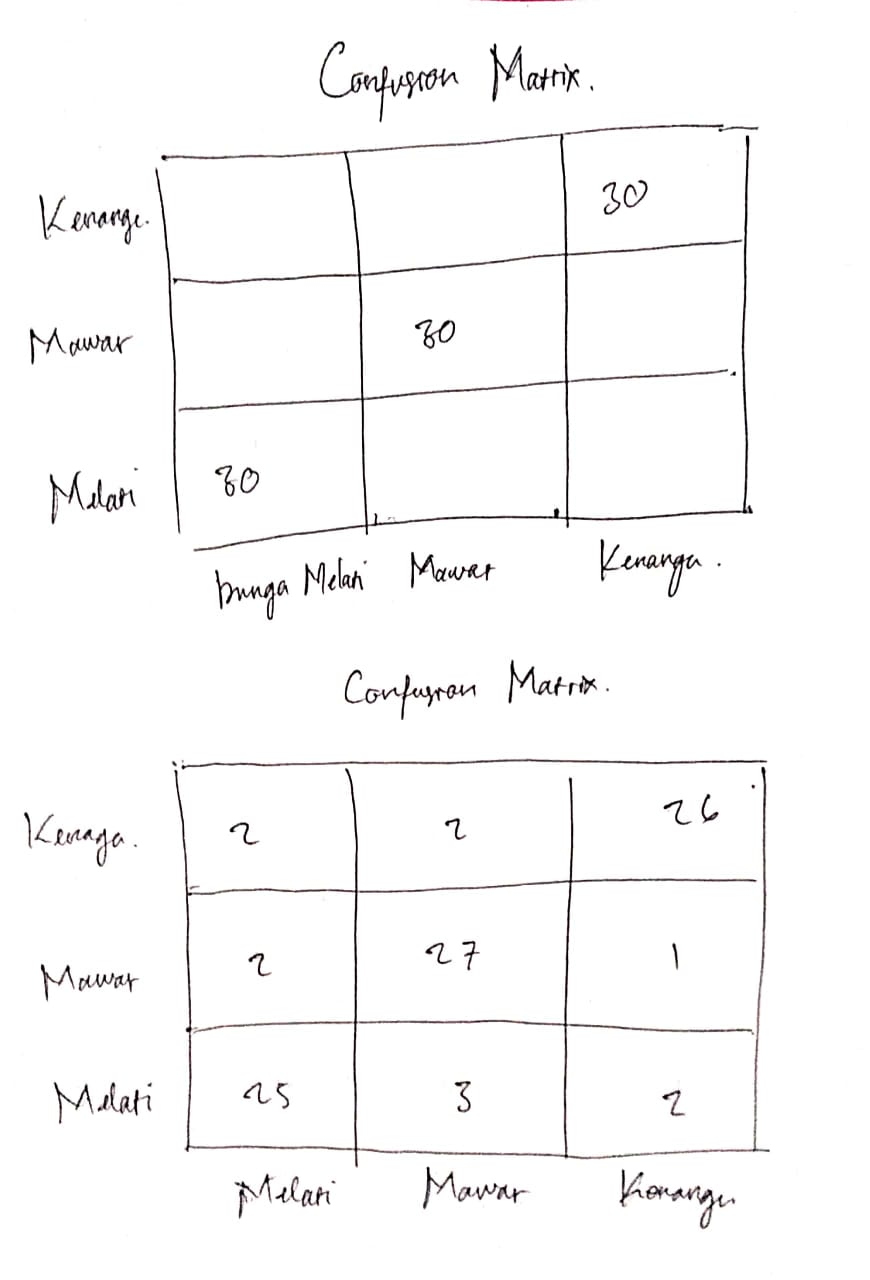
\includegraphics[width=1\textwidth]
      {figures/c15}}
      \caption{Contoh Binary Classification}
      \label{c15}
      \end{figure}

\begin{figure}[ht]
      \centerline{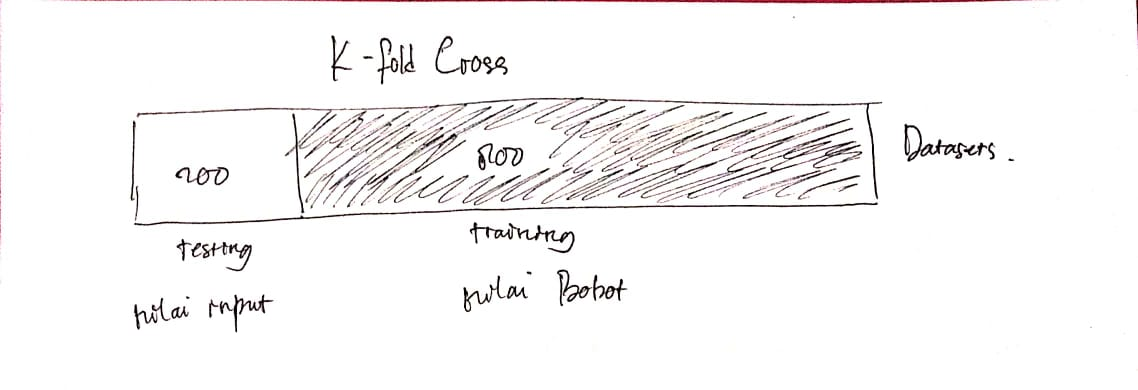
\includegraphics[width=1\textwidth]
      {figures/c16}}
      \caption{Contoh Binary Classification}
      \label{c16}
      \end{figure}

\begin{figure}[ht]
      \centerline{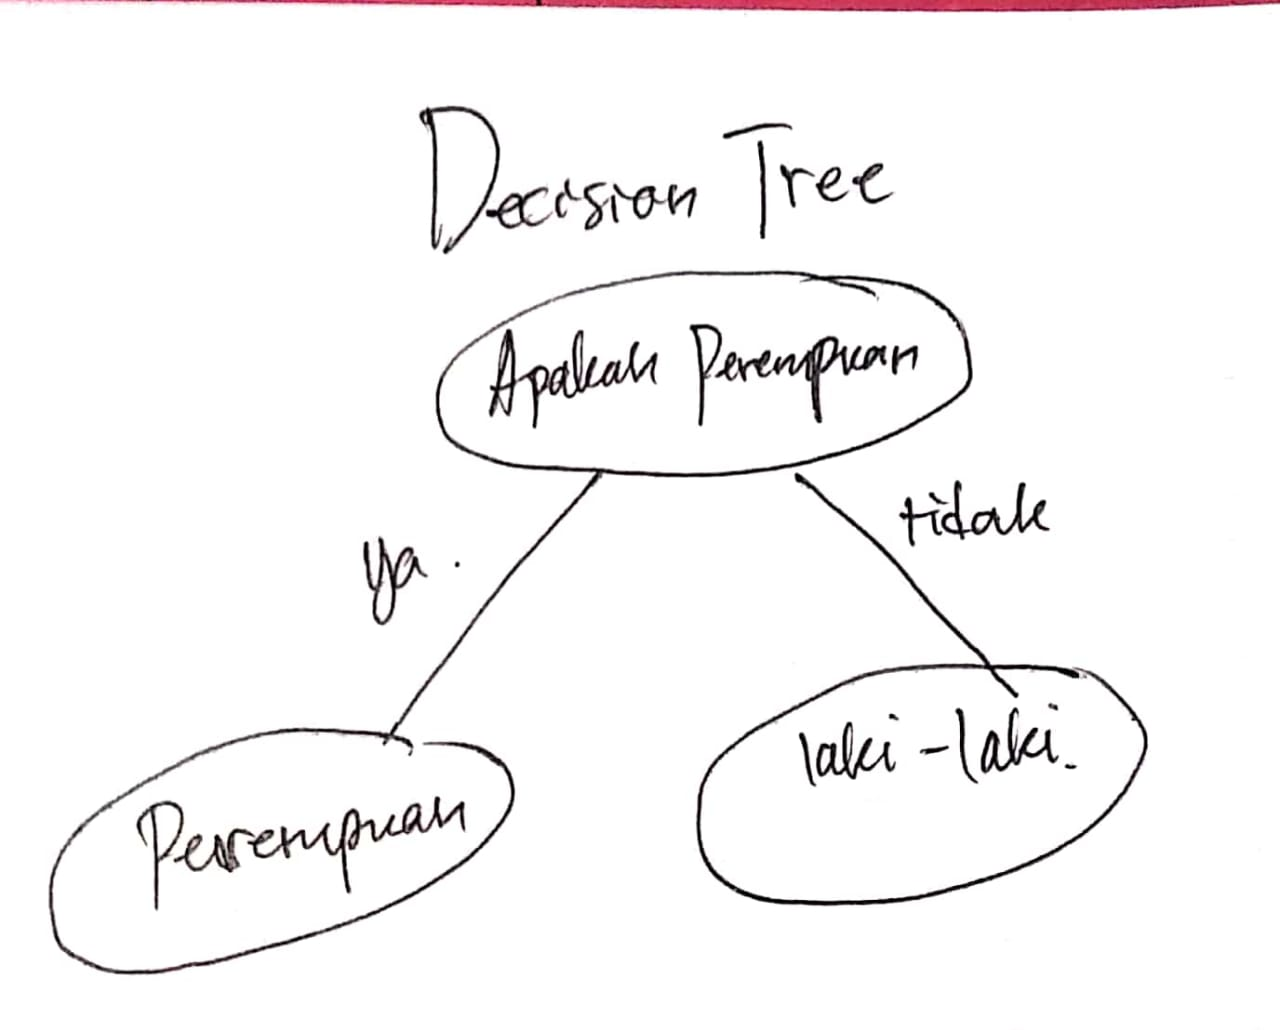
\includegraphics[width=1\textwidth]
      {figures/c17}}
      \caption{Contoh Binary Classification}
      \label{c17}
      \end{figure}

\begin{figure}[ht]
      \centerline{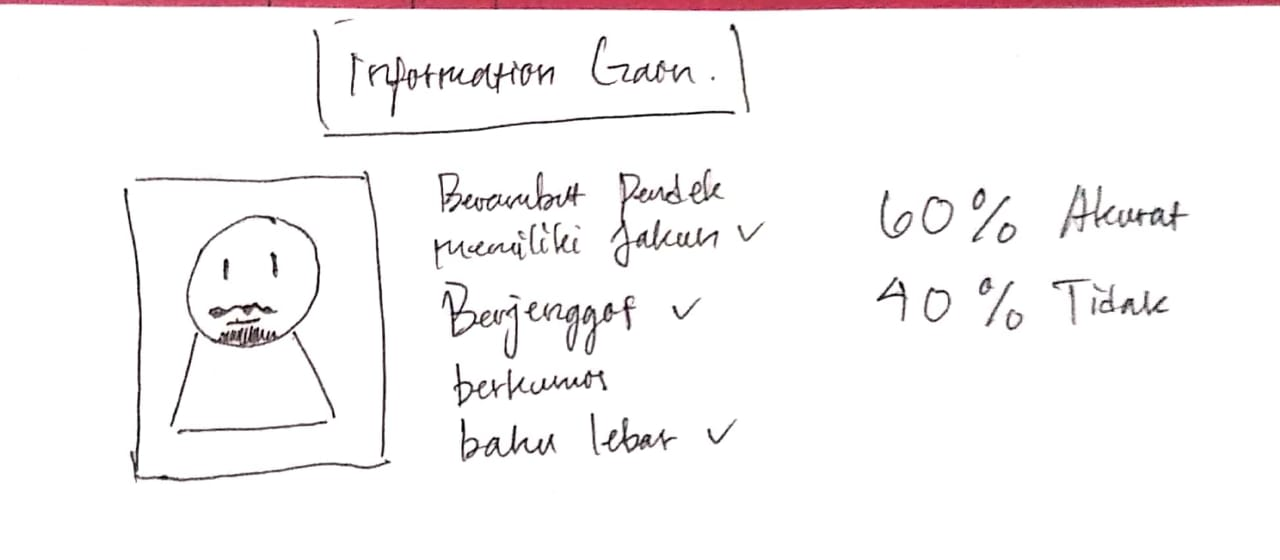
\includegraphics[width=1\textwidth]
      {figures/c18}}
      \caption{Contoh Binary Classification}
      \label{c18}
      \end{figure}


 